\documentclass{anstrans}
%%%%%%%%%%%%%%%%%%%%%%%%%%%%%%%%%%%
\title{NekRS: Massively parallel fluid flow simulations in reactor cores}
\author{Paul Fischer,$^{*}$ Stefan Kerkemeier,$^{\dagger}$ Yu-Hsiang Lan,$^{\dagger}$ Misun Min, $^{\dagger}$ and Elia Merzari $^{\ddagger}$}

\institute{
$^{*}$ University of Illinois at Urbana-Champaign, fischerp@illinois.edu
\and
$^{\dagger}$ Argonne National Laboratory
\and
$^{\ddagger}$ Pennsylvania State University
}

% Optional disclaimer: remove this command to hide
%\disclaimer{Notice: this manuscript is a work of fiction. Any resemblance to
%actual articles, living or dead, is purely coincidental.}

%%%% packages and definitions (optional)
\usepackage{graphicx} % allows inclusion of graphics
\usepackage{booktabs} % nice rules (thick lines) for tables
\usepackage{microtype} % improves typography for PDF

\newcommand{\SN}{S$_N$}
\renewcommand{\vec}[1]{\bm{#1}} %vector is bold italic
\newcommand{\vd}{\bm{\cdot}} % slightly bold vector dot
\newcommand{\grad}{\vec{\nabla}} % gradient
\newcommand{\ud}{\mathop{}\!\mathrm{d}} % upright derivative symbol

\begin{document}
%%%%%%%%%%%%%%%%%%%%%%%%%%%%%%%%%%%%%%%%%%%%%%%%%%%%%%%%%%%%%%%%%%%%%%%%%%%%%%%%
\section{Introduction}

Computational fluid dynamics has achieved  widespread use both in reactor design and in safety analysis, as testified by the increasing number of articles in the field. Among recent examples, Roelofs \cite{roelofs2018thermal} illustrates the importance of CFD for liquid metal reactor design and analysis. In fact, detailed modeling and simulation is of particular importance for advanced reactors,  where it can be used in conjunction with separate effect experiments, until integral test data is available.

Reynolds Averaged Navier-Stokes (RANS) and occasionally Unsteady Reynolds Averaged Navier Stokes (URANS) remain the workhorse for analysis conducted in industry, research centers, and academia.  However, despite significant advancements in turbulence modeling in recent years, RANS is limited in terms of accuracy.   In contrast to RANS, Wall-resolved Large Eddy simulation (LES) and Direct Numerical Simulation (DNS) provide a much lesser degree of uncertainty, and they can provide valuable and unprecedented insight into the flow physics.

Thanks to the the advent of Petascale computing (i.e, computers capable of more than 1 Petaflop), the simulation of portions of nuclear components has been demonstrated with LES \cite{merzari2020}. For example, the simulation of large portions of fuel assemblies has been demonstrated:  these simulations can provide invaluable insight into the flow dynamics, which is difficult or often impossible to obtain with experiments alone. Moreover, they allow investigation of global effects that otherwise are impossible to elucidate with smaller portions of the system. NEAMS has put considerable resources into scalable high-order CFD software that can leverage large scale supercomputers to deliver simulations of unprecedented detail and scale.

Even with Petascale computing, limitations in nuclear modeling and simulation tools remain. Resolution requirements limit our capacity to reach higher Reynolds numbers, for instance. Time-scale separation also limits severely our capacity to simulate transient behavior. Nonetheless, the continued increase in computational resources is enabling a further expansion of what can be simulated. The main driver of the transition to Exascale (i.e, computers capable of more than 1 Exaflop) will inevitably be weak scaling \cite{merzari2017large}. Simulations of significant portions of a reactor core with LES are now on the horizon at moderate Reynolds numbers (up to $Re=50,000$).

In order to exploit the power of Exascale and pre-Exascale architectures in the
United States,  however, performant GPU implementations of computational fluid
dynamics algorithms are needed. In this manuscript we summarize recent efforts
to port the spectral element code Nek5000 \cite{fischer2015nek5000} to GPUs. In
particular we discuss a novel version of the code, NekRS, and a series of large
scale simulations performed on ORNL's Summit, the second largest supercomputer
in the world. These simulations demonstrate the potential of NekRS to simulate
large portions of the reactor core and showcase the excellent performance of
the code on Summit.

\section{Nek5000 and NekRS}

Nek5000 \cite{fischer2015nek5000} is an open-source simulation software package
that delivers highly accurate solutions for a wide range of scientific
applications, including fluid flow, thermal convection, combustion, and
magnetohydrodynamics. It features state-of-the-art, scalable high-order
algorithms that are fast and efficient on platforms ranging from laptops to the
DOE leadership computing facilities.

Nek5000 is based on the spectral element method \cite{patera1984} in which the
domain is decomposed globally into smaller domains (elements), which are
assumed to be curvilinear hexahedra (brick meshes) conforming to the domain
boundaries. Locally, functions within each element are expanded in high-order
(typically $N=4$--12) tensor-product polynomials. The pressure can be solved
at the same polynomial order as the velocity $N$ ($P_{N} - P_{N}$ formulation)
or at lower order $N-2$ ($P_{N} - P_{N-2}$ formulation). Temporal
discretization is based on a high-order splitting that is third-order accurate
in time and reduces the coupled velocity-pressure Stokes problem to four
independent solves per timestep: one for each velocity component and one for
the pressure. The velocity problems are diagonally dominant and thus easily
solved by using Jacobi preconditioned conjugate gradient iteration. Two
timestepping schemes, both up to third order, are available: semi-implicit
BDF-extrapolation or subcycle-based characteristics. The characteristics
scheme permits relatively large timesteps corresponding to CFL numbers
of 4 or more \cite{patel19}, but is typically run as a second-order
scheme to reduce advection-subcycle-evaluation cost.  Each Navier-Stokes
timestep requires a pressure-Poisson solve, which is effected through
multigrid-preconditioned GMRES iteration coupled with temporal projection to
find an optimal initial guess.  Particularly important components of Nek5000
are its scalable coarse-grid solvers that are central to parallel performance.
For both weak and strong scaling, using algebraic multigrid for the coarse-grid
solve is essential above 250,000 elements. Nek5000 employs a pure MPI parallel
implementation. An extensive discussion of the scalability of Nek5000 is
provided in \cite{fischer15,fischer20a}.

NekRS is a new GPU-oriented version of Nek5000  that is also capable of running
on CPUs. It represents a significant redesign of the code. While written in
C++, NekRS is able to link to Nek5000 to leverage its extensive pre- and
postprocessing utilities. NekRS has been built primarily under the auspices of
the DOE Exascale Computing Project.  NekRS relies on a native GPU library,
libParanumal \cite{libP}, for highly-performant kernels to evaluate (and
solve) the PDE operators.  The main kernels require fast evaluation of the 
Laplacian (for the viscous Helmholtz solves for each velocity component and
for the pressure-Poisson solve), fast preconditioners (for pressure), and
fast, fully dealiased, advection operators.  The coarse-grid pressure solves
are performed either with parAlmond from the libParanumal library or with
Hypre.


\section{Selected results}

The rapid convergence of the high-order discretizations in Nek5000 and NekRS
and their high performance on the DOE's leadership computing facilities makes
them ideally suited for LES/DNS in complex domains.  Here, we present performance
results related to the flow in light-water small modular reactors and
in pebble beds.

\subsection{Flow in a 17x17 assembly and extension to full core}

We discuss here weak-scaling studies performed on Summit for a 17x17 assembly
and multi-assembly calculations performed with NekRS. Figure~\ref{fig:gpu2}
shows results for a 17x17 rod bundle LES calculation; this simulation (selected
results are presented in \cite{merzari2020}) has been scaled up to 75 billion
grid-points for moderate Reynolds numbers and full core conditions.

We analyze in more detail here the performance of NekRS vs. Nek5000 for fuel
assemblies. Figure~\ref{fig:nekrs1}, left, shows strong scaling results on a
few nodes of Summit using NekRS with six V100 GPUs per node or NekRS/Nek5000
with 42 CPUs per node for the 17x17 case. For the CPU version, NekRS uses Hypre
as a coarse grid solver. In this case, NekRS is about 4X slower than Nek5000
because the pressure solver is not yet as optimized as the highly-tuned solver
in Nek5000. For the GPU, the NekRS results improve substantially when the
coarse grid solver is based on the AMG solver ParAlmond.
Figure~\ref{fig:nekrs1} , center, shows the pressure iteration counts for each
of the four cases. Nek5000 uses Schwarz-smoothed p-multigrid; NekRS uses
Chebyshev smoothing. When ParAlmond is used for the coarse-grid solve the NekRS
iteration counts improve by a factor of two and are on par with those of
Nek5000. The Chebyshev smoother requires more work per iteration than the
Schwarz-based smoother. With ongoing effort on the pressure solve we anticipate
a 2X reduction in NekRS solution times, which will put it on par with the
strong-scaled solution times of Nek5000 with more than 2X energy savings that
are already observed for NekRS on Summit's V100s (Figure~\ref{fig:nekrs1} ,
right).

Table~\ref{wscaling2} shows results for the weak scaling performance on Summit for NekRS for 17x17 assembly calculations (8,000 elements per GPU, $N=7$), with increasing mesh counts. The axial length was simply extended while keeping the mesh resolution the same. We note that the time per time-step stabilizes quickly indicating a good weak-scaling performance even for this more complex case.

We note that a full core calculation was also performed with 150 million elements and the average time for time step was 0.7s.

\begin{figure}[!ht]
\centering
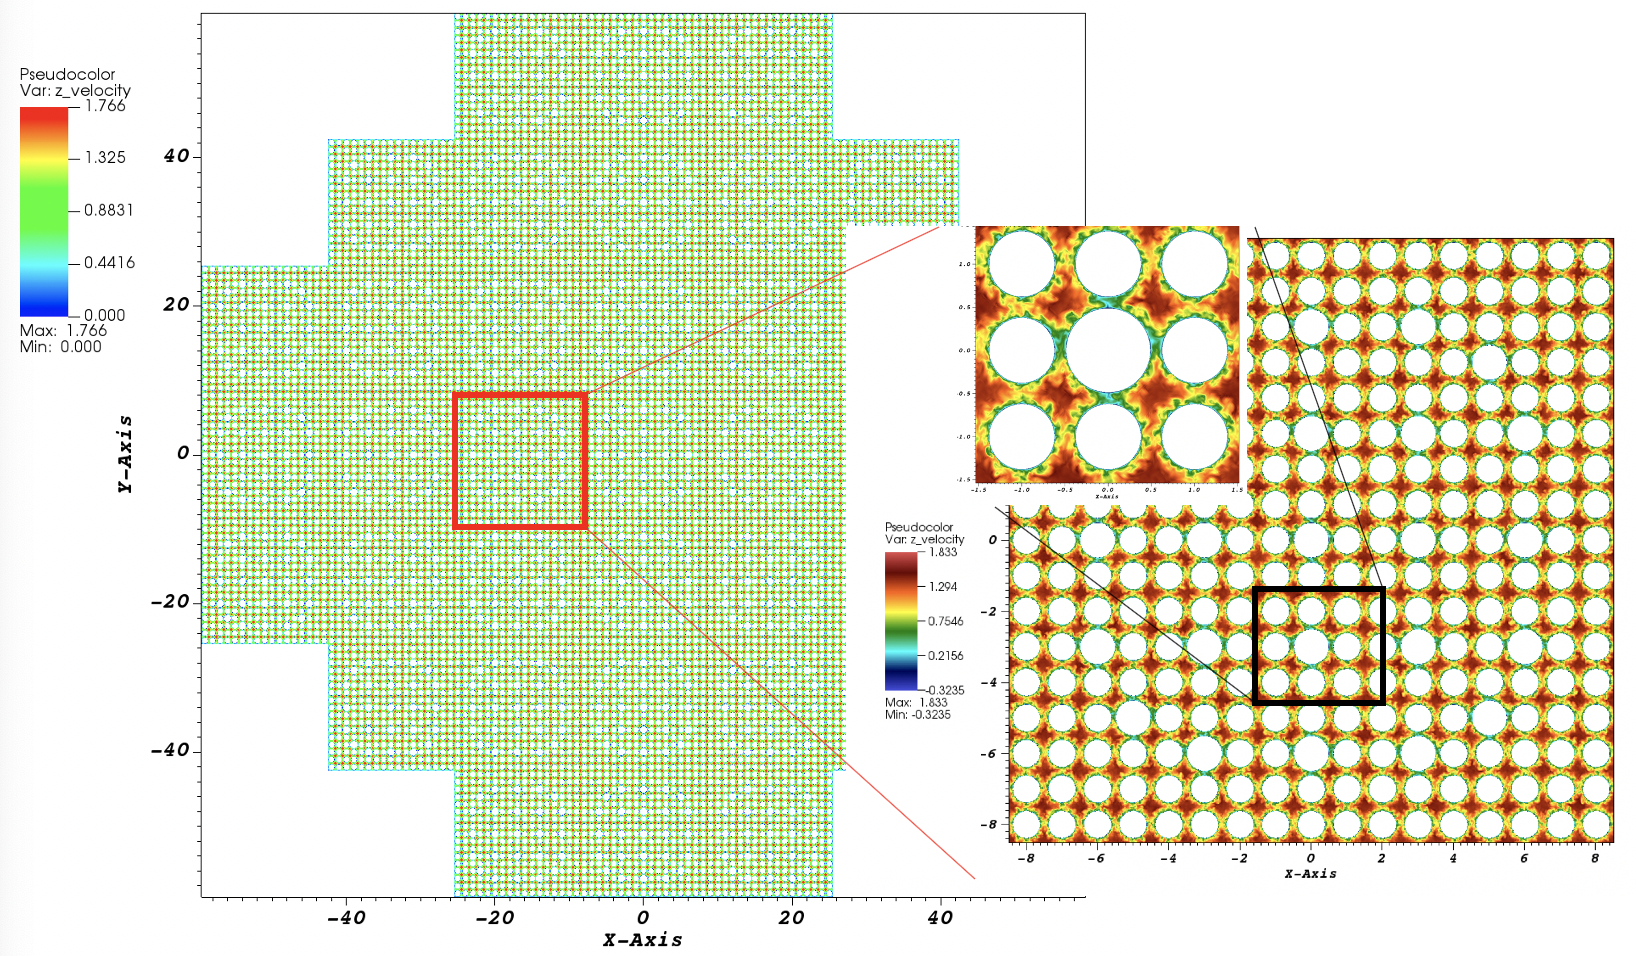
\includegraphics[width=0.5\textwidth]{./Figures/full_core_summary.png}
\caption{Numerical simulation of a full core SMR calculation and in a 17x17 assembly. (left) full core. (right) LES simulation in a 17x17 assembly}
\label{fig:gpu2}
\end{figure}

\begin{figure}[h]
\centering
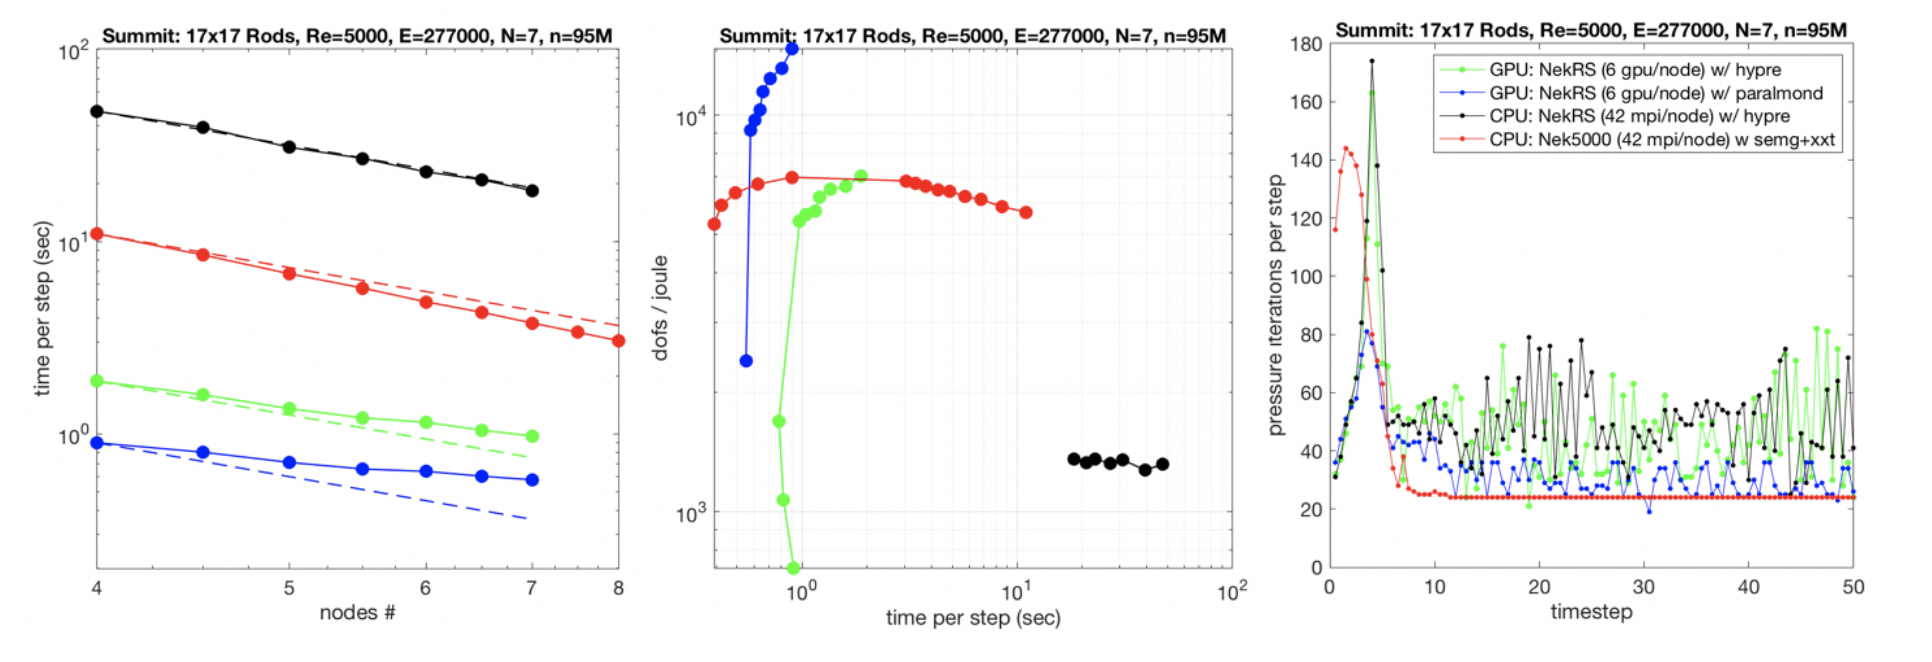
\includegraphics[width=0.5\textwidth]{./Figures/performance_nekrs}
\caption{ NekRS and Nek5000 performance of GPUs vs. CPUs on Summit for turbulent flow simulations with Re=5000 for a 17x17 rod-bundle geometry using total number of grid points $n=95,011,000$. Based on timings from Step 11 to 60, time-per-step with ideal scalings shown as dashed lines (left), pressure iterations per step (center), and dofs-per-joule with respect to time-per-step (right) are shown.}
\label{fig:nekrs1}
\end{figure}


\begin{table} [!b]
\resizebox{0.48\textwidth}{!}{
 \begin{tabular}{ccc}
\# of Nodes on Summit & Elements (Million) & Average time per time-step \\
\midrule
6	 & 0.277	& 0.312 s \\
66  & 3 	  & 0.455 s \\
264  & 12	  & 0.648 s \\
660  & 30	  & 0.506 s \\
\bottomrule \end{tabular} }
\caption{\label{wscaling2} Weak-scaling on Summit for 17x17 assembly case.}
\end{table}


\subsection{Pebble bed cores}

We have recently developed an all-hex meshing tool for flow around
dense-packed spheres that is ideal for studying the thermal-hydraulics
of pebble-bed reactors.  The meshing strategy is built upon the Voronoi
cells associated with the pebble centers in which each Voronoi facet is
tessellated into quadrilaterals that are projected onto the sphere surfaces.
The swept hexahedral volumes are partitioned in the radial direction to
provide more resolution and the overall mesh is smoothed to yield a 
well-conditioned mesh that minimizes excessive CFL constaints.

Figures~\ref{f:ndemo3} and ~\ref{f:ndemo4} illustrate the type of
domains that are accessible with this approach.  
  Table~\ref{tab:pebble} reports the number of pebbles and number
of elements per pebble for several test cases.
The largest case to date, comprising 11,145 pebbles, uses 3.5 million
spectral elements of degree $N=7$ with a total of 
$n := EN^3$ = 2 billion grid points for Reynolds number $Re_D=5000$.

\begin{figure}[!h]
\centering
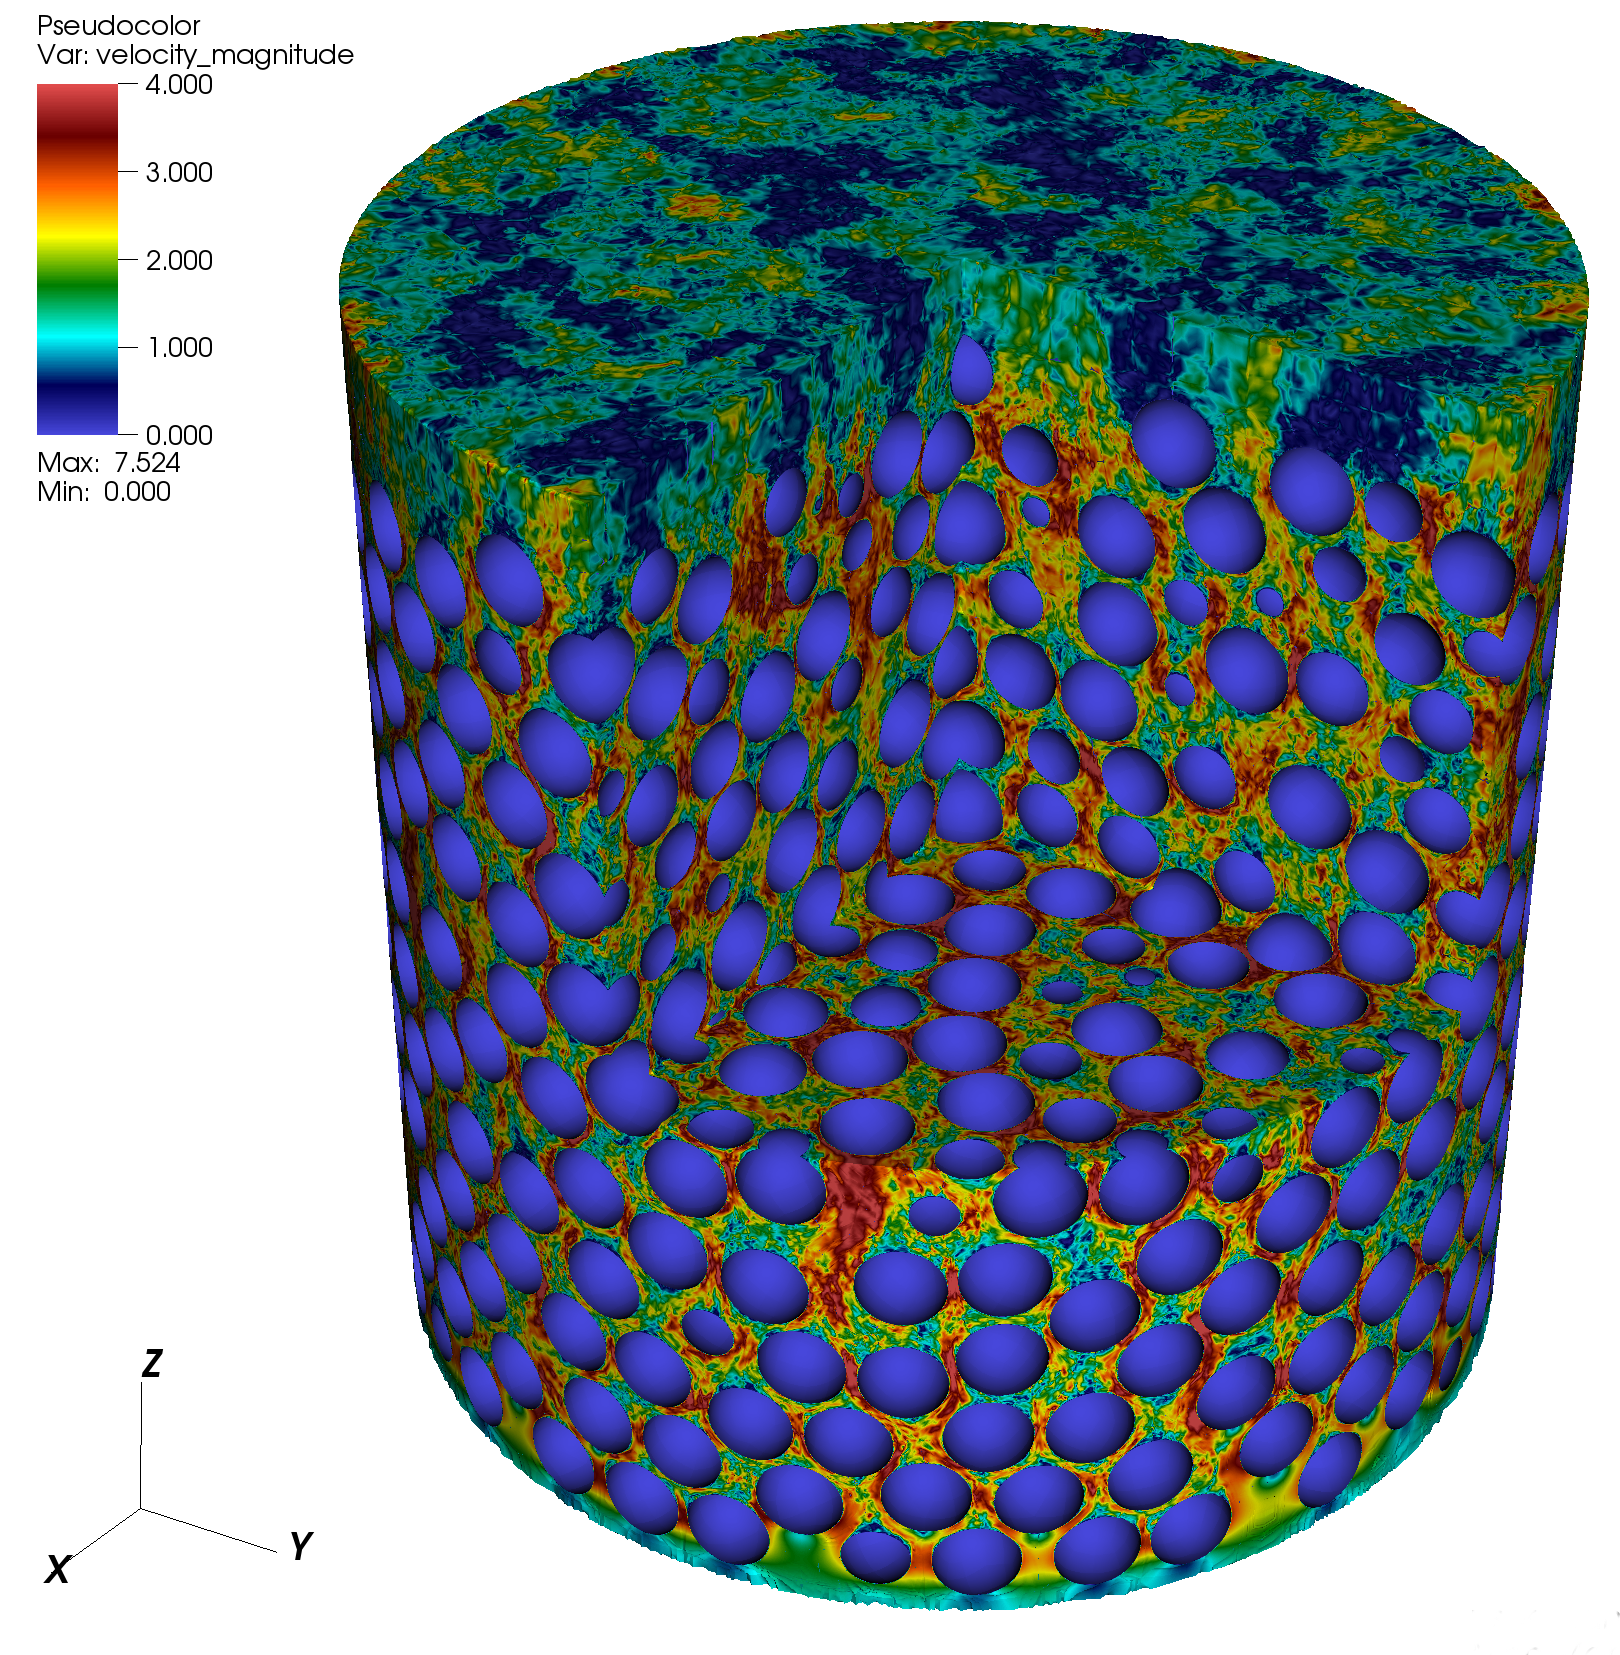
\includegraphics[clip=true,width=0.4\textwidth]{Figures/ndemo_r3}
\caption{NekRS: a velocity component for turbulent flow simulations using the
spectral element mesh with 524,386 spectral elements for 1568 pebbles. }
\label{f:ndemo3}
\end{figure}

\begin{figure}[!h]
\centering
\includegraphics[clip=true,width=0.4\textwidth]{Figures/peb3260}
\caption{NekRS: a velocity component for turbulent flow simulations using the
spectral element mesh with 1,121,214 spectral elements for 3260 pebbles. }
\label{f:ndemo4}
\end{figure}


 \begin{table} \centering \small
% \resizebox{0.48\textwidth}{!}{
  \begin{tabular}{ccc} \hline \hline
   \# pebbles & $E$ & $E$/pebble \\ \hline
  146 & 62,132 & 425 \\
  1568 & 524,386 & 334 \\
  3260 & 1,121,214 & 343 \\
  11145 & 3,575,076 & 320 \\ \hline \hline
 \end{tabular}%}
% \begin{tabular}{cccccccc}
% \hline \hline
%  \# pebbles & $E$ & $E$/pebble & \# nodes & \# GPUs & $E$/GPU & $n$/GPU & walltime/step (s) \\
% \hline
% 146 & 62,132 & 425 & 2 & 12 & 5177 & 2.6M & 0.34  \\
% 1568 & 524,386 & 334 & 28 & 168 & 3121 & 1.5M & 0.40  \\
% 3260 & 1,121,214 & 343 & 50 & 300 & 3737 & 1.9M & 0.75  \\
% 11145 & 3,575,076 & 320 & 148 & 888 & 4025 & 2.0M & 0.90 \\
%  \hline \hline
%\end{tabular}}
  \caption{NekRS: All-hex meshes for pebbles based on Voronoi cell strategy.}
  \label{tab:pebble}
 \end{table}

We also examine strong-scaling performance of NekRS (GPU) and NekRS
(CPU) in Table~\ref{tab:nekrs1}. We measured timings for 100 timesteps for
turbulent flow simulations with the 1568-pebble mesh on ORNL's Summit, using 42
MPI ranks per node for the CPU runs and 6 Nvidia V100s per node for the GPU
runs. For the same node count, the GPU-accelerated variant of NekRS is more
than 9$\times$ faster when using 3.5 million points per GPU (here, 7283
spectral elements per GPU and $N=7$). The NekRS GPU run realizes 82\%
parallel efficiency at 2.1 million points per GPU.

\begin{table}
 \resizebox{0.48\textwidth}{!}{
 \begin{tabular}{c|cccc||cccc}
  \hline
 % \multirow{2}{*}{ } &
 \multicolumn{1}{c|}{ } &
 \multicolumn{4}{|c||}{NekRS GPU} &
 \multicolumn{4}{|c}{NekRS CPU} \\
 \hline
 %\cline{2-5}
  Nodes & $E$/GPU & $n$/GPU & walltime/step (s) & eff & $E$/MPI& $n$/MPI & walltime/step (s) & eff\\
 \hline
  12 & 7283 & 2.4M & 0.569 & 1.00 & 1040 & 356K & 5.361 & 1.00\\
  20 & 4369 & 1.4M & 0.416 & 0.82 & 624 & 214K & 3.055 & 1.05\\
  28 & 3121 & 1.0M & 0.338 & 0.72 & 445 & 152K & 2.200 & 1.04\\
  36 & 2427 & 0.8M & 0.309 & 0.61 & 346 & 118K & 1.876 & 0.95\\
  44 & 1986 & 0.6M & 0.290 & 0.53 & 283 & 97K & 1.401 & 1.04\\
  52 & 1680 & 0.5M & 0.255 & 0.51 & 240 & 82K & 1.204 & 1.02\\
  \hline \hline
\end{tabular}}
 \caption{NekRS GPU/CPU Strong-Scale Timings (seconds per step) for 100 Steps
of Turbulent flow Simulations with $Re=10000$ for 1568-Pebble Case Using Total
Number of Grid Points $n=179,864,398$ ($E=524,386$ and $N=7$).}
 \label{tab:nekrs1}
\end{table}

\section{Conclusions}

In this summary we have examined large scale simulations on Summit using the
new GPU spectral element solver NekRS, a port of Nek5000. The simulations
clearly demonstrate the potential of Nek5000 to be applied to full core
calculations.

For example for pebble beds, twenty nodes represents less than 1\% of the
computing power available on Summit, which is sufficient for 1568 pebbles at
2.1 million points per GPU. Performance throughput for NekRS saturates at 2--4
million points per GPU on Summit. By running with 4 million points per GPU, we
estimate that 80\% of the machine will be sufficient to perform a full-core
calculation in FHRs corresponding to 300,000 pebbles.

\bibliographystyle{ans}
\bibliography{references}
\end{document}
